\documentclass[a4paper]{article}

%% Language and font encodings
\usepackage[english]{babel}
\usepackage[utf8x]{inputenc}
\usepackage[T1]{fontenc}

%% Sets page size and margins
\usepackage[a4paper,top=3cm,bottom=2cm,left=3cm,right=3cm,marginparwidth=1.75cm]{geometry}

%% Useful packages
\usepackage{amsmath}
\usepackage{graphicx}
\usepackage[colorinlistoftodos]{todonotes}
\usepackage[colorlinks=true, allcolors=blue]{hyperref}

\title{CPA Lab 2}
\author{Carlos Santiago Galindo Jiménez\\Jesús Vélez Palacios}

\begin{document}
\maketitle
\section{Objective}
Parallelize the execution of a program that reconstructs an image whose rows have been shuffled. Study different approaches and some improvements to the algorithm.




\begin{figure}[h]
    \centering
    \begin{tabular}{l r}
        Program            & Execution time \\ \hline
        \texttt{encaja-e1} & 15.257217      \\
        \texttt{encaja-e3} &  2.725587      \\
    \end{tabular}
    \caption{Sequential execution times}
\end{figure}
\begin{figure}[h]
    \centering
    \begin{tabular}{l r r r r r}
        Program               & 2t        & 4t        & 8t        & 16t        & 32t        \\ \hline
        \texttt{encaja-e2-pJ} & 6.938746  & 3.548883  & 1.970450  & 1.183996   & 0.726187   \\
        \texttt{encaja-e2-pX} & 8.337415  & 5.464151  & 5.557857  & 8.197272   & 12.789012  \\
        \texttt{encaja-e4-pJ} & 1.439842  & 0.795035  & 0.496000  & 0.330912   & 0.256960   \\
        \texttt{encaja-e4-pX} & 4.065065  & 4.217589  & 5.164125  & 8.656438   & 13.590685  \\
    \end{tabular}
    \caption{Parallel execution times}
\end{figure}

\begin{figure}[h]
    \centering
    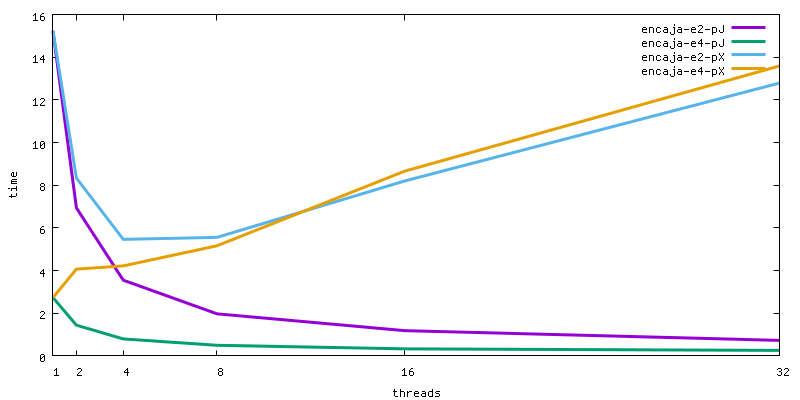
\includegraphics[width=\textwidth]{img/time}
    \caption{Threads\, \textemdash\unskip \, time graph}
\end{figure}
\end{document}
